% Options for packages loaded elsewhere
\PassOptionsToPackage{unicode}{hyperref}
\PassOptionsToPackage{hyphens}{url}
%
\documentclass[
  man,floatsintext]{apa6}
\usepackage{amsmath,amssymb}
\usepackage{iftex}
\ifPDFTeX
  \usepackage[T1]{fontenc}
  \usepackage[utf8]{inputenc}
  \usepackage{textcomp} % provide euro and other symbols
\else % if luatex or xetex
  \usepackage{unicode-math} % this also loads fontspec
  \defaultfontfeatures{Scale=MatchLowercase}
  \defaultfontfeatures[\rmfamily]{Ligatures=TeX,Scale=1}
\fi
\usepackage{lmodern}
\ifPDFTeX\else
  % xetex/luatex font selection
\fi
% Use upquote if available, for straight quotes in verbatim environments
\IfFileExists{upquote.sty}{\usepackage{upquote}}{}
\IfFileExists{microtype.sty}{% use microtype if available
  \usepackage[]{microtype}
  \UseMicrotypeSet[protrusion]{basicmath} % disable protrusion for tt fonts
}{}
\makeatletter
\@ifundefined{KOMAClassName}{% if non-KOMA class
  \IfFileExists{parskip.sty}{%
    \usepackage{parskip}
  }{% else
    \setlength{\parindent}{0pt}
    \setlength{\parskip}{6pt plus 2pt minus 1pt}}
}{% if KOMA class
  \KOMAoptions{parskip=half}}
\makeatother
\usepackage{xcolor}
\usepackage{graphicx}
\makeatletter
\def\maxwidth{\ifdim\Gin@nat@width>\linewidth\linewidth\else\Gin@nat@width\fi}
\def\maxheight{\ifdim\Gin@nat@height>\textheight\textheight\else\Gin@nat@height\fi}
\makeatother
% Scale images if necessary, so that they will not overflow the page
% margins by default, and it is still possible to overwrite the defaults
% using explicit options in \includegraphics[width, height, ...]{}
\setkeys{Gin}{width=\maxwidth,height=\maxheight,keepaspectratio}
% Set default figure placement to htbp
\makeatletter
\def\fps@figure{htbp}
\makeatother
\setlength{\emergencystretch}{3em} % prevent overfull lines
\providecommand{\tightlist}{%
  \setlength{\itemsep}{0pt}\setlength{\parskip}{0pt}}
\setcounter{secnumdepth}{-\maxdimen} % remove section numbering
% Make \paragraph and \subparagraph free-standing
\ifx\paragraph\undefined\else
  \let\oldparagraph\paragraph
  \renewcommand{\paragraph}[1]{\oldparagraph{#1}\mbox{}}
\fi
\ifx\subparagraph\undefined\else
  \let\oldsubparagraph\subparagraph
  \renewcommand{\subparagraph}[1]{\oldsubparagraph{#1}\mbox{}}
\fi
\newlength{\cslhangindent}
\setlength{\cslhangindent}{1.5em}
\newlength{\csllabelwidth}
\setlength{\csllabelwidth}{3em}
\newlength{\cslentryspacingunit} % times entry-spacing
\setlength{\cslentryspacingunit}{\parskip}
\newenvironment{CSLReferences}[2] % #1 hanging-ident, #2 entry spacing
 {% don't indent paragraphs
  \setlength{\parindent}{0pt}
  % turn on hanging indent if param 1 is 1
  \ifodd #1
  \let\oldpar\par
  \def\par{\hangindent=\cslhangindent\oldpar}
  \fi
  % set entry spacing
  \setlength{\parskip}{#2\cslentryspacingunit}
 }%
 {}
\usepackage{calc}
\newcommand{\CSLBlock}[1]{#1\hfill\break}
\newcommand{\CSLLeftMargin}[1]{\parbox[t]{\csllabelwidth}{#1}}
\newcommand{\CSLRightInline}[1]{\parbox[t]{\linewidth - \csllabelwidth}{#1}\break}
\newcommand{\CSLIndent}[1]{\hspace{\cslhangindent}#1}
\ifLuaTeX
\usepackage[bidi=basic]{babel}
\else
\usepackage[bidi=default]{babel}
\fi
\babelprovide[main,import]{english}
% get rid of language-specific shorthands (see #6817):
\let\LanguageShortHands\languageshorthands
\def\languageshorthands#1{}
% Manuscript styling
\usepackage{upgreek}
\captionsetup{font=singlespacing,justification=justified}

% Table formatting
\usepackage{longtable}
\usepackage{lscape}
% \usepackage[counterclockwise]{rotating}   % Landscape page setup for large tables
\usepackage{multirow}		% Table styling
\usepackage{tabularx}		% Control Column width
\usepackage[flushleft]{threeparttable}	% Allows for three part tables with a specified notes section
\usepackage{threeparttablex}            % Lets threeparttable work with longtable

% Create new environments so endfloat can handle them
% \newenvironment{ltable}
%   {\begin{landscape}\centering\begin{threeparttable}}
%   {\end{threeparttable}\end{landscape}}
\newenvironment{lltable}{\begin{landscape}\centering\begin{ThreePartTable}}{\end{ThreePartTable}\end{landscape}}

% Enables adjusting longtable caption width to table width
% Solution found at http://golatex.de/longtable-mit-caption-so-breit-wie-die-tabelle-t15767.html
\makeatletter
\newcommand\LastLTentrywidth{1em}
\newlength\longtablewidth
\setlength{\longtablewidth}{1in}
\newcommand{\getlongtablewidth}{\begingroup \ifcsname LT@\roman{LT@tables}\endcsname \global\longtablewidth=0pt \renewcommand{\LT@entry}[2]{\global\advance\longtablewidth by ##2\relax\gdef\LastLTentrywidth{##2}}\@nameuse{LT@\roman{LT@tables}} \fi \endgroup}

% \setlength{\parindent}{0.5in}
% \setlength{\parskip}{0pt plus 0pt minus 0pt}

% Overwrite redefinition of paragraph and subparagraph by the default LaTeX template
% See https://github.com/crsh/papaja/issues/292
\makeatletter
\renewcommand{\paragraph}{\@startsection{paragraph}{4}{\parindent}%
  {0\baselineskip \@plus 0.2ex \@minus 0.2ex}%
  {-1em}%
  {\normalfont\normalsize\bfseries\itshape\typesectitle}}

\renewcommand{\subparagraph}[1]{\@startsection{subparagraph}{5}{1em}%
  {0\baselineskip \@plus 0.2ex \@minus 0.2ex}%
  {-\z@\relax}%
  {\normalfont\normalsize\itshape\hspace{\parindent}{#1}\textit{\addperi}}{\relax}}
\makeatother

% \usepackage{etoolbox}
\makeatletter
\patchcmd{\HyOrg@maketitle}
  {\section{\normalfont\normalsize\abstractname}}
  {\section*{\normalfont\normalsize\abstractname}}
  {}{\typeout{Failed to patch abstract.}}
\patchcmd{\HyOrg@maketitle}
  {\section{\protect\normalfont{\@title}}}
  {\section*{\protect\normalfont{\@title}}}
  {}{\typeout{Failed to patch title.}}
\makeatother

\usepackage{xpatch}
\makeatletter
\xapptocmd\appendix
  {\xapptocmd\section
    {\addcontentsline{toc}{section}{\appendixname\ifoneappendix\else~\theappendix\fi\\: #1}}
    {}{\InnerPatchFailed}%
  }
{}{\PatchFailed}
\keywords{Affect, Speech, Voice, Machine Learning, Mobile Sensing\newline\indent Word count: 5464}
\usepackage{csquotes}
\ifLuaTeX
  \usepackage{selnolig}  % disable illegal ligatures
\fi
\IfFileExists{bookmark.sty}{\usepackage{bookmark}}{\usepackage{hyperref}}
\IfFileExists{xurl.sty}{\usepackage{xurl}}{} % add URL line breaks if available
\urlstyle{same}
\hypersetup{
  pdftitle={AI-Based Recognition of Affect Experience from Speech Collected with Smartphones},
  pdfauthor={Timo K. Koch1,2, Gabriella M. Harari3, Ramona Schoedel2, Zachariah Marrero4, Florian Bemmann5, Samuel D. Gosling4, Markus Buehner2, \& Clemens Stachl1},
  pdflang={en-EN},
  pdfkeywords={Affect, Speech, Voice, Machine Learning, Mobile Sensing},
  hidelinks,
  pdfcreator={LaTeX via pandoc}}

\title{AI-Based Recognition of Affect Experience from Speech Collected with Smartphones}
\author{Timo K. Koch\textsuperscript{1,2}, Gabriella M. Harari\textsuperscript{3}, Ramona Schoedel\textsuperscript{2}, Zachariah Marrero\textsuperscript{4}, Florian Bemmann\textsuperscript{5}, Samuel D. Gosling\textsuperscript{4}, Markus Buehner\textsuperscript{2}, \& Clemens Stachl\textsuperscript{1}}
\date{}


\shorttitle{Affect Experience in Speech}

\authornote{

Conflict of interest: none
Acknowledgements: We thank Peter Ehrich and Dominik Heinrich for their support with the technical implementation of the on-device acoustic feature extraction for study 1. We thank ZPID for the support with data collection for study 1. Thanks Sumer Vaid for technical support in the analyses of study 2. This project was supported by a scholarship of the German Academic Scholarship Foundation awarded to the first author.

The authors made the following contributions. Timo K. Koch: Conceptualization, Formal Analysis, Writing - Original Draft Preparation, Writing - Review \& Editing; Gabriella M. Harari: Writing - Review \& Editing, Supervision; Ramona Schoedel: Conceptualization, Writing - Review \& Editing; Zachariah Marrero: Data curation; Florian Bemmann: Software; Samuel D. Gosling: Resources; Markus Buehner: Resources; Clemens Stachl: Writing - Review \& Editing, Supervision.

Correspondence concerning this article should be addressed to Timo K. Koch, Postal address. E-mail: \href{mailto:timo.koch@unisg.ch}{\nolinkurl{timo.koch@unisg.ch}}

}

\affiliation{\vspace{0.5cm}\textsuperscript{1} Institute of Behavioral Science and Technology, University of St.~Gallen\\\textsuperscript{2} Department of Psychology, Ludwig-Maximilians-Universität München\\\textsuperscript{3} Stanford University\\\textsuperscript{4} University of Texas\\\textsuperscript{5} Media Informatics Group, Ludwig-Maximilians-Universität München}

\abstract{%
Advances in the area of artificial intelligence (AI) and the ubiquity of speech data, for example coming from voice assistants, have created numerous commercial products that claim to be able to automatically recognize emotions from human speech. However, the employed algorithms have often been trained solely on enacted or labelled speech samples from artificial lab settings representing affect \emph{expression} and are used to infer everyday subjective affect \emph{experience}. In the present work, we investigate if machine learning algorithms can truly recognize subjective affect experience from speech samples collected in the wild. In two studies, we extract acoustic voice parameters and state-of-the-art word embeddings from 23632 speech samples with corresponding experience-sampled self-reports on momentary affect experience from 1066 participants collected using off-the-shelf smartphones. While voice acoustics provide limited predictive information of affective arousal, speech content is predictive of arousal as well as valence (sadness and contentedness). Further, experimental and explorative findings suggest that emotional speech content does not affect predictions from voice acoustics (i.e., what someone talks about does not affect how well emotions can be predicted from voice cues alone). We discuss implications for the algorithmic monitoring of affect experience from speech in everyday life.
}



\begin{document}
\maketitle

\hypertarget{introduction}{%
\subsection{Introduction}\label{introduction}}

Research findings on the algorithmic recognition of affective states (e.g., emotions) and related affective disorders from speech offer promising applications, for instance in health care, human-machine interaction, education, and marketing (Hildebrand et al., 2020; Milling, Pokorny, Bartl-Pokorny, \& Schuller, 2022). The advances in algorithmic affect recognition from speech leveraging AI and the ubiquity of available speech data due to the rise of voice assistants, for example Amazon's Alexa and Apple's Siri, have created an increasing commercial interest in the field. Here, tech companies aim to leverage speech data to, for instance, recognize what momentary affect their customers experience in order to develop personalized user interfaces or make product recommendations (Knight, 2016; Mandell, 2020; Vlahos, 2019). Most of the prediction models used in research and in the corresponding commercial tools are trained on enacted or labelled speech samples from artificial lab settings that represent emotion \emph{expressions}. However, those algorithms are often deployed to detect people's subjective affect \emph{experience} in everyday life. Further, many of the commercial algorithms are not transparent with regard to how well their predictions work and how (biased) predictions are being made. These issues raise questions regarding the promises of emotion-detecting speech technology and the protection of user privacy in setting where speech data can be analyzed, for example, when using voice assistants. The present work investigates the algorithmic recognition of between-person differences and within-person fluctuations in subjective self-reported momentary affect \emph{experience} from speech samples collected with smartphones.

\hypertarget{predicting-affect-from-speech}{%
\subsubsection{Predicting Affect from Speech}\label{predicting-affect-from-speech}}

Researchers have successfully predicted affective states from a range of speech data, such as labelled TV clips (Grimm, Kroschel, \& Narayanan, 2008), phone calls, and enacted speech samples from the lab (Bänziger, Mortillaro, \& Scherer, 2012; Burkhardt, Paeschke, Rolfes, Sendlmeier, \& Weiss, 2005; Schuller, 2018; Vogt, André, \& Wagner, 2008). They report on impressive prediction performances for the automatic recognition of emotions (i.e., correlations between true scores and predicted scores of up to .81 for arousal and .68 for valence predictions) (Weninger, Eyben, Schuller, Mortillaro, \& Scherer, 2013). However, one has to keep in mind that in those works the enacted target emotion or the rater labels serve as ground truth. Thereby, these works predict affect \emph{expression}, which is considered easier to algorithmically recognize than real-life \emph{experienced} affect (Vogt et al., 2008). Moreover, the prediction performance varies greatly across studies due to a varying choice of emotion targets (i.e., discrete emotion versus core affect), conceptualizations of affect (e.g., short-termed elicited emotions versus moods), and employed algorithms (e.g., supervised versus unsupervised machine learning).

Also, these prior studies on algorithmic affect recognition often offer no insights into how predictions in their ``black box'' models were being made. For instance, it frequently remains unclear which specific speech characteristics are particularly predictive of a given affective state. Prior descriptive research reported on associations of specific acoustic features and affective states. For example, voice pitch and intensity were found to be associated with affective arousal (Vogt et al., 2008; Weninger et al., 2013). Two recent studies provide a remarkable non-technical summary of voice features (Hildebrand et al., 2020) and a comprehensive overview of associations of word use with affect in spoken language (Sun, Schwartz, Son, Kern, \& Vazire, 2020). Recent developments in the area of interpretable machine learning can help gain insights into the inner working of machine learning algorithms and, consequently, aid with detecting speech features that are especially predictive of affective states (Molnar, 2019).

Due to the challenge of obtaining speech data with corresponding affect labels in-vivo, most prior research on affect recognition from speech has used actors or labelled samples. This comes with a set of downsides, such as actors potentially overacting and the ambiguity of ground truth due to the subjective nature of labeling (Batliner et al., 2011; Schuller, 2018; Wilting, Krahmer, \& Swerts, 2006). As a consequence, studies investigating predictions of subjective affect experience from speech are rare. Recent works have collected everyday speech samples using the Electronically Activated Recorder (EAR) (Mehl, 2017). Hereby, speech data can be collected over a period of time which allows researchers to not only investigate between-person differences in affect (i.e., is this person sad?), but also assess within-person fluctuations (i.e., is this person sadder than other days?) (Huang \& Epps, 2018; Sun et al., 2020; Weidman et al., 2020). Using the EAR, however, can be privacy invasive since potentially non-consenting persons may be recorded, too. Moreover, handling the EAR recorders and transmitting the collected data can be tedious for participants and researchers.
Here, off-the-shelf smartphones represent a useful platform to collect experience samples on momentary affect experience over time and make corresponding speech records using the build-in microphone (Carlier et al., 2022; Sun et al., 2020; Weidman et al., 2020).

\hypertarget{content-form-interactions-in-affect-recognition-from-speech}{%
\subsubsection{Content-Form Interactions in Affect Recognition from Speech}\label{content-form-interactions-in-affect-recognition-from-speech}}

Prior research has shown that voice form (prosody) and the lexical content of the produced words (semantics) work together when transmitting affective information through speech (Ben-David, Multani, Shakuf, Rudzicz, \& van Lieshout, 2016). Moreover, studies suggest that there is a prosodic (i.e., from voice cues) dominance in the perception of affect based on lab experiments (Ben-David et al., 2016; Lin, Ding, \& Zhang, 2020), but not (yet) using speech data from the wild (Schwartz \& Pell, 2012). Moreover, while this research field had focused on the interplay of prosody and semantics in the recognition of affect by human raters, there are, to our knowledge, no studies on content-form interactions in algorithmic affect detection. Hence, it is currently unclear if what users talk about (i.e., the emotional content) has an effect on voice acoustics that impact automated affect recognition. In an applied setting, for example, the question is if an algorithm could recognize affective states regardless of what the person talks about, may it be a mundane topic, such as the weather or ordering pizza, or does one need to talk about an emotional topic (e.g., meeting a loved one).

The present work leverages methodological advances in the area of smartphone-based data collection methods to investigate the prediction of between-person differences and within-person fluctuations in subjective momentary affect experience from speech. In two large-scale studies, we train cross-validated machine learning models on acoustic voice cues and state-of-the-art word embeddings from speech samples collected in the wild. Moreover, for predictive models, we investigate which voice cues are most predictive. Further, we experimentally and exploratively investigate the effects of the emotionality of speech's content on algorithmic affect recognition from voice acoustics. Thereby, we aim to inform potential applications and promises in automatic affect recognition from speech signals and advise the discussion on the protection of user privacy rights.

\hypertarget{study-1}{%
\subsection{Study 1}\label{study-1}}

\hypertarget{method}{%
\subsubsection{Method}\label{method}}

\hypertarget{smartphone-based-voice-data-collection-and-privacy-preserving-on-device-acoustic-feature-extraction}{%
\paragraph{Smartphone-Based Voice Data Collection and Privacy-Preserving On-Device Acoustic Feature Extraction}\label{smartphone-based-voice-data-collection-and-privacy-preserving-on-device-acoustic-feature-extraction}}

Data collection for this study was part of a large six-month panel study (from May until November 2020) using the \emph{PhoneStudy} research app at Ludwig-Maximilian-Universität München (Schoedel \& Oldemeier, 2020). Data collection was approved by the responsible IRB board. The study comprised two two-week experience sampling phases (July 27, 2020, to August 9,2020; September 21, 2020, to October 4, 2020) during which participants received two to four short questionnaires per day. Here, self-reported valence and arousal were assessed in two separate items on six-point Likert scales among other psychological properties as part of an experience sampling procedure. Furthermore, for each experience sampling instance, we computed the fluctuation of assessed momentary affect in valence and arousal from one's (median) affect baseline (for participants with at the five experience sampling days) across all experience sampling instances. For example, if a participant had a valence baseline of ``3'' and reports a ``6'' in a particular moment, this fluctuation score of ``+3'' indicated that this person had been a lot more happy than usual.

The last experience sampling questionnaire of each day included an additional instruction, where participants were asked to read out a series of predefined emotional sentences while making an audio recording of their voice. The sentences presented to the participants are based on a set of validated German neutral and affective sentences (Defren et al., 2018) and differ in their emotional content: positive (e.g., ``My team won yesterday.''), negative (e.g., ``Nobody is interested in my life.''), and neutral (e.g., ``The plate is on the round table.''). These three emotional categories are presented consecutively in each audio logging task. The order of the categories was randomized per experience sampling questionnaire. For each emotional content category, three sentences were randomly drawn from respective sets of sentences in the database. The use and experimental manipulation of these emotional semantic categories allowed us to control for the content spoken by our participants and at the same time enabled us to conduct a privacy-friendly study. The audio recording was started by the participants via a button on the screen. Participants could stop the recording manually after a minimum of four seconds. Alternatively, the recording was stopped automatically after twelve seconds. We chose these lower- and upper-time thresholds because this is the minimum and maximum time required to read out the three sentences per condition.
Once the audio record had been completed, we used the widely adopted \emph{OpenSMILE} open-source algorithm (Eyben, Wöllmer, \& Schuller, 2010) to automatically extract acoustic features directly on the participant's device. Here, we used the extended Geneva Minimalistic Acoustic Parameters Set (eGeMAPS) that is comprised of 88 acoustic features (Eyben et al., 2016). Theses voice feature have been used in a range of prior studies on affect recognition from speech. After feature extraction, the voice records were automatically deleted and only extracted voice features were stored on our servers.

With this procedure, we collected 11199 audio logs from 586 participants. We excluded 214 voice logs because the respective acoustic features (mean voicing score, voiced segments per second, mean voiced segment length) indicated that no human voice was recorded. Moreover, we excluded a total of 997 samples without corresponding self-reports on valence and arousal, from participants with less than five experience sampling days, and those participants who had no variance in all their valence and arousal scores across all their experience samples.
This left us with a final data set of 9908 voice samples with corresponding acoustic features from 3381 experience sampling instances for valence and arousal from 499 participants (48.50\% female, \emph{M}(Age) = 42.97 years). Overall self-reported valence was positive (\emph{M} = 4.72, \emph{SD} = 1.03) and overall arousal was slightly geared towards activity (\emph{M} = 3.68, \emph{SD} = 1.35). The distribution of valence and arousal as well as fluctuations from the baseline is provided in the online supplements.

In the final sample, voice samples were not equally distributed across emotional sentence conditions (\emph{chi}\textsuperscript{2}(2) = 36.48, \emph{p} \textless{} .001): 3219 came from the positive condition, 3110 from the neutral condition, and 3579 from the negative condition.

\hypertarget{predictive-modelling}{%
\paragraph{Predictive Modelling}\label{predictive-modelling}}

We trained multiple supervised machine learning models on the extracted acoustic voice features for the prediction of self-reported valence and arousal and their fluctuations. Here, we compared the predictive performance of linear regularized regression models (LASSO) (Zou \& Hastie, 2005) with those of a non-linear tree-based Random Forest model (Breiman, 2001; Wright \& Ziegler, 2017), and a baseline model. The baseline model would predict the respective mean values for valence and arousal of the respective training set for all cases in a test set. Additionally, we included the prediction of participants' age and gender as a benchmark. Models were evaluated using a ten-fold cross-validation scheme (Bischl, Mersmann, Trautmann, \& Weihs, 2012). We blocked participants in the resampling procedure ensuring that for each train/test set pair the given participant is either in the training set or in the test set.

We evaluated the predictive performance of the models based on the coefficient of determination (\emph{R}\textsuperscript{2}) and Spearman's (rank) correlation (\emph{r}) between the predicted scores and participants' self-reported scores. To determine whether a model was predictive beyond chance (\emph{alpha} = 0.05), we carried out variance-corrected (one-sided) t-tests comparing the \emph{R}\textsuperscript{2} measures of all prediction models with those of the baseline models (Nadeau \& Bengio, 2003). We adjusted for multiple comparison (\emph{n} = 8) via Holm correction.

All data processing and statistical analyses in this work were performed with the statistical software R version 4.1.1 (R Core Team, 2021). For machine learning, we used the \emph{mlr3} framework (Lang et al., 2019). Specifically, we used the \emph{glmnet} (Friedman, Hastie, \& Tibshirani, 2010) and \emph{ranger} (Wright \& Ziegler, 2017) packages to fit prediction models. To quantify the impact of single predictors in Random Forest prediction models, we computed (out-of-bag) permutation feature importance using the \emph{DALEX} package (Biecek, 2018; Wright, Ziegler, \& König, 2016). We preregistered the present study as a transparent account of our work (Koch \& Schoedel, 2021).

\hypertarget{results}{%
\subsubsection{Results}\label{results}}

\hypertarget{recognizing-affect-experience-from-acoustic-voice-cues}{%
\paragraph{Recognizing Affect Experience from Acoustic Voice Cues}\label{recognizing-affect-experience-from-acoustic-voice-cues}}

Overall, none of the employed machine learning algorithms predicted affect experience on the dimensions of valence and arousal significantly better than chance, even though, on average, predictions of raw arousal scores (\emph{R}\textsuperscript{2} = , \emph{r} = ) and arousal fluctuations (\emph{R}\textsuperscript{2} = , r = ) from Random Forest models were slightly better than the baseline models' predictions. On the contrary, valence predictions did not yield any predictive information. Figure \ref{fig:gerpredictionoverview} provides an overview of the performance of all employed machine learning algorithms across prediction tasks. In the arousal prediction tasks, Random Forest models performed slightly better than LASSO models, suggesting non-linear relationships between voice cues and affective arousal outcomes in the present study. Finally, benchmark predictions of speaker age (\emph{R}\textsuperscript{2} = 0.11, \emph{r} = 0.39) and gender (prediction accuracy = 91.40\%) suggest that voice acoustics from the collected read-out sentences in Study 1 contain valuable information about speaker demographics.

\begin{figure}

{\centering 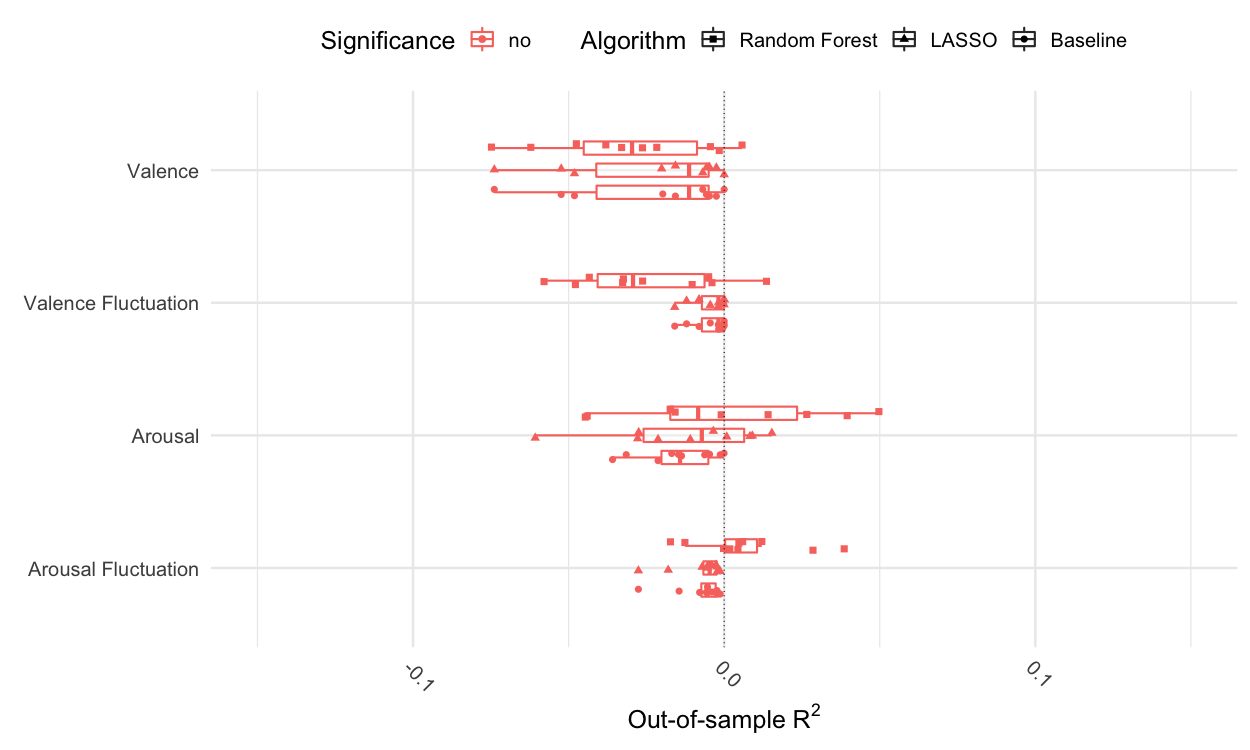
\includegraphics[width=1\linewidth,height=0.45\textheight]{../figures/bmr_ger_egemaps_plot} 

}

\caption[Prediction performance Study 1]{Box and whisker plot of prediction performance measures from 10-fold cross-validation for prediction models.}\label{fig:gerpredictionoverview}
\end{figure}

\hypertarget{content-effects-on-affect-predictions-from-voice-acoustics}{%
\paragraph{Content Effects on Affect Predictions from Voice Acoustics}\label{content-effects-on-affect-predictions-from-voice-acoustics}}

Finally, we analyzed if the experimentally altered emotional content (positive/ neutral/ negative) of the predefined sentences that had been read out by participants had an effect on affect predictions from voice acoustics. Here, we focused on predictions of between-person differences in valence and arousal since these showed a better, even though not significant, prediction performance than those models for within-person fluctuations. There were no significant differences in prediction errors across the three sentence conditions for valence (\emph{F}(2,11873) = 0.09,
\emph{p} \textgreater{} .05) and arousal (\emph{F}(2,11873) = 0.39,
\emph{p} \textgreater{} .05) predictions suggesting that sentences' emotional valence did not influence affect predictions from voice acoustics (see Figure \ref{fig:gercontenteffect}).

\begin{figure}

{\centering 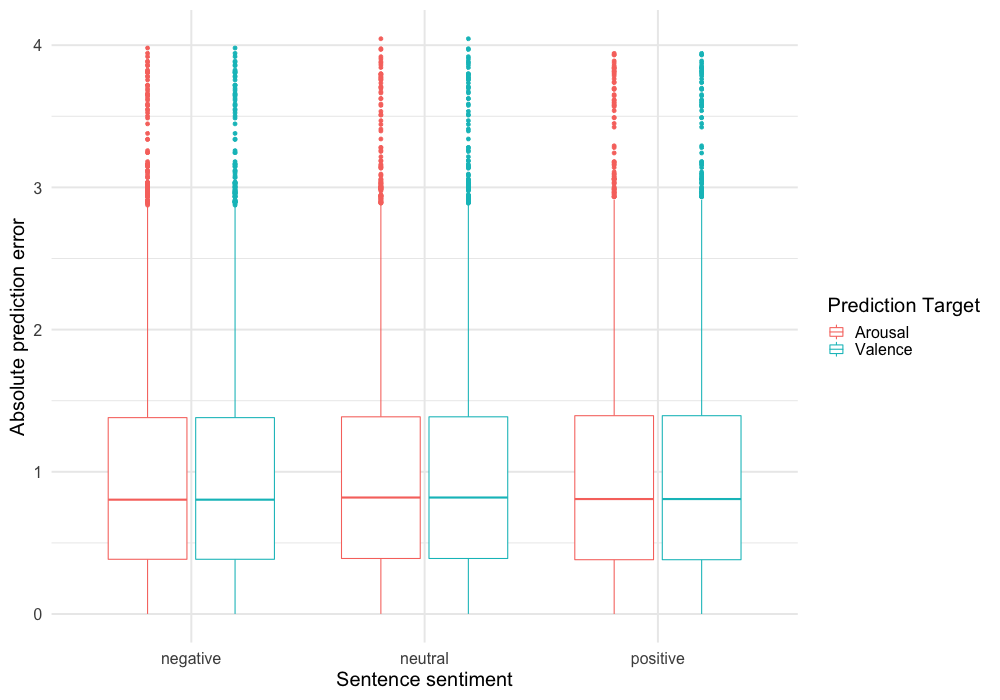
\includegraphics[width=1\linewidth]{../figures/predictions_condition_plot} 

}

\caption[Prediction error in different emotional sentence conditions]{Prediction error for valence and arousal prediction in Random Forest models from voice acoustics in different emotional sentence conditions.}\label{fig:gercontenteffect}
\end{figure}

\newpage

\hypertarget{study-2}{%
\subsection{Study 2}\label{study-2}}

\hypertarget{method-1}{%
\subsubsection{Method}\label{method-1}}

\hypertarget{smartphone-based-speech-data-collection}{%
\paragraph{Smartphone-Based Speech Data Collection}\label{smartphone-based-speech-data-collection}}

Data collection for this study was part of the UT1000 Project at the University of Texas at Austin in the United States in fall 2018 (Wu et al., 2021). During a three-week self-tracking assignment using their smartphones, students from a Synchronous Massive Online Course (SMOC) in introductory psychology received four short experience sampling questionnaires per day where they could also make records of their speech at the end. Here, self-reported arousal (assessed on a five-point Likert scale), contentedness, and sadness were assessed in separate items on four-point Likert scales among other psychological properties as part of an experience sampling procedure. Thereby, in Study 2, we captured emotional valence on two items (contentedness and sadness) instead of one as done in Study 1. According to the affect grid, contentedness and sadness have a comparable low level of arousal and an opposing emotional valence. Furthermore, for each experience sampling instance, in line with Study 1., we computed the fluctuation of assessed momentary affect in arousal, contentedness, and sadness from one's (median) affect baseline (for participants with at least five experience sampling days) across all experience sampling instances.
For the audio records, participants received the following instruction: ``Please record a short audio clip in which you describe the situation you are in, and your current thoughts and feelings. Collect about 10 seconds of environmental sound after the description.'' The responses to this prompt are analyzed in the present study. Any parts of the record that did not contain speech were cut out before further analysis since the focus of this work is affect in human speech. The collected speech samples had also been used in another research project that describes the data collection procedure in more detail (Marrero, Gosling, Pennebaker, \& Harari, 2022).

With this procedure, we collected 23482 audio logs from 980 participants. We followed the same procedure to select speech records as in Study 1 and, to ensure comparability of the two studies with regard to the length of speech samples, we retained all speech transcripts that contained at least 15 words and were more than four seconds long which is equivalent to the length of the sentences that had been read out in Study 1: We removed records where the respective acoustic features indicated that no human voice was recorded. Moreover, we excluded audio samples without corresponding affect self-reports, participants with less than five experience sampling days, and those participants who had no variance in all their valence and arousal scores across all their experience samples.

This procedure left us with a final data set of 13724 speech samples with corresponding experience-sampled self-reports on momentary affect experience from 567 participants (64.90\% female, \emph{M}(Age) = 18.57 years). Overall participants reported balanced experienced contentedness (\emph{M} = 1.65, \emph{SD} = 0.85) and low sadness (\emph{M} = 0.53, \emph{SD} = 0.77). Overall arousal was balanced out (\emph{M} = 1.95, \emph{SD} = 0.95). The distribution of arousal, contentedness, and sadness as well as respective fluctuations from the baseline is provided in the online supplements.

In the same manner as in Study 1, we extracted the extended Geneva Minimalistic Acoustic Parameters Set (eGeMAPS) from the collected audio files using the OpenSMILE algorithm (Eyben et al., 2016, 2010). In Study 2, those features were extracted from the raw recorded audio files after data collection and not directly on participants' smartphones as in Study 1.

We transcribed all raw audio records using the Google Speech-to-text API. Then, we extracted state-of-the-art word embeddings from speech transcripts using the \emph{text} R package (Kjell, Giorgi, \& Schwartz, 2021). Word embeddings are vector representations of words in a high-dimensional space, which capture their meaning and relationships with other words. Specifically, for predictive modeling, we used the second to last layer (layer 23) from the language model ``RoBERTa large'' as recommended in prior work (Liu et al., 2019; Matero, Hung, \& Schwartz, 2022).

\hypertarget{predictive-modelling-1}{%
\paragraph{Predictive Modelling}\label{predictive-modelling-1}}

For predictive modelling, we applied the same machine learning pipeline using the same R packages as used in Study 1 to predict self-reported sadness, contentedness, and arousal as well as their deviations from the respective person's baseline levels. Moreover, in addition to extracted acoustic features, we also used extracted word embeddings as features. To investigate and compare the predictive power of speech form (voice cues) and content (word embeddings), we ran predictions on all features combined as well as acoustic features and word embeddings separately.

\hypertarget{results-1}{%
\subsubsection{Results}\label{results-1}}

\hypertarget{prediction-of-affect-experience-from-speech}{%
\paragraph{Prediction of Affect Experience from Speech}\label{prediction-of-affect-experience-from-speech}}

The employed machine learning models trained on voice acoustics (speech form) and word embeddings (speech content) predicted between-person differences and within-person fluctuations in the subjective experience of momentary affect experience significantly better than chance. Figure \ref{fig:uspredictionoverview} provides an overview of the performance of all learners across prediction tasks while in this section we report on the best performing algorithm respectively (either Random Forest or LASSO).
Our models yielded the best prediction performance for between-person variations in contentedness (\emph{R}\textsuperscript{2} = 0.10, \emph{r} = 0.34), arousal (\emph{R}\textsuperscript{2} = 0.09, \emph{r} = 0.32), and sadness (\emph{R}\textsuperscript{2} = 0.04, \emph{r} = 0.24). Also, for within-person fluctuations, predictions were significantly better than chance for contentedness (\emph{R}\textsuperscript{2} = 0.06, \emph{r} = 0.26), arousal (\emph{R}\textsuperscript{2} = 0.05, \emph{r} = 0.22), and sadness (\emph{R}\textsuperscript{2} = 0.02, \emph{r} = 0.13). However, overall, predictions were better for between-person differences than for within-person fluctuations.

Moreover, evaluation prediction performance of models trained only on voice acoustics or word embedding respectively revealed that predictions were mostly driven by the information coming from speech content as represented in the word embeddings. Prediction models trained on voice acoustics alone were not significantly better than chance. However, on average, predictions of between-person differences in contentedness (\emph{R}\textsuperscript{2} = 0.01, \emph{r} = 0.14) and arousal (\emph{R}\textsuperscript{2} = 0, \emph{r} = 0.12) as well as arousal fluctuations (\emph{R}\textsuperscript{2} = 0, \emph{r} = 0.12) were slightly better than the baseline models' predictions.

Prediction models trained on word embeddings were significantly predictive of all affective states: Between-person differences in arousal (\emph{R}\textsuperscript{2} = 0.09, \emph{r} = 0.31), contentedness (\emph{R}\textsuperscript{2} = 0.10, \emph{r} = 0.33), and sadness (\emph{R}\textsuperscript{2} = 0.06, \emph{r} = 0.23) as well as within-person fluctuations of arousal (\emph{R}\textsuperscript{2} = 0.05, \emph{r} = 0.22), contentedness (\emph{R}\textsuperscript{2} = 0.06, \emph{r} = 0.26), and sadness (\emph{R}\textsuperscript{2} = 0.02, \emph{r} = 0.13).

For voice acoustics, as in Study 1, the Random Forest algorithm performed slightly better than the LASSO algorithm, suggesting non-linear relationships between voice cues and affect experience. On the contrary, for word embeddings, LASSO models performed better than Random Forest models, indicating linear predictor-outcome relationships between speech content as captured with word embeddings and momentary affect experience.

Finally, while predictions of speaker age were not better than chance (\emph{R}\textsuperscript{2} = -0.19, \emph{r} = 0.08) for any of the feature sets, likely due to the low age variance in the data set, gender predictions yielded very good prediction results (prediction accuracy = 95.76\%). These findings suggest that voice acoustics and speech content from the collected semi-structured speech samples in Study 2 contain valuable information about speaker demographics.

\begin{figure}

{\centering 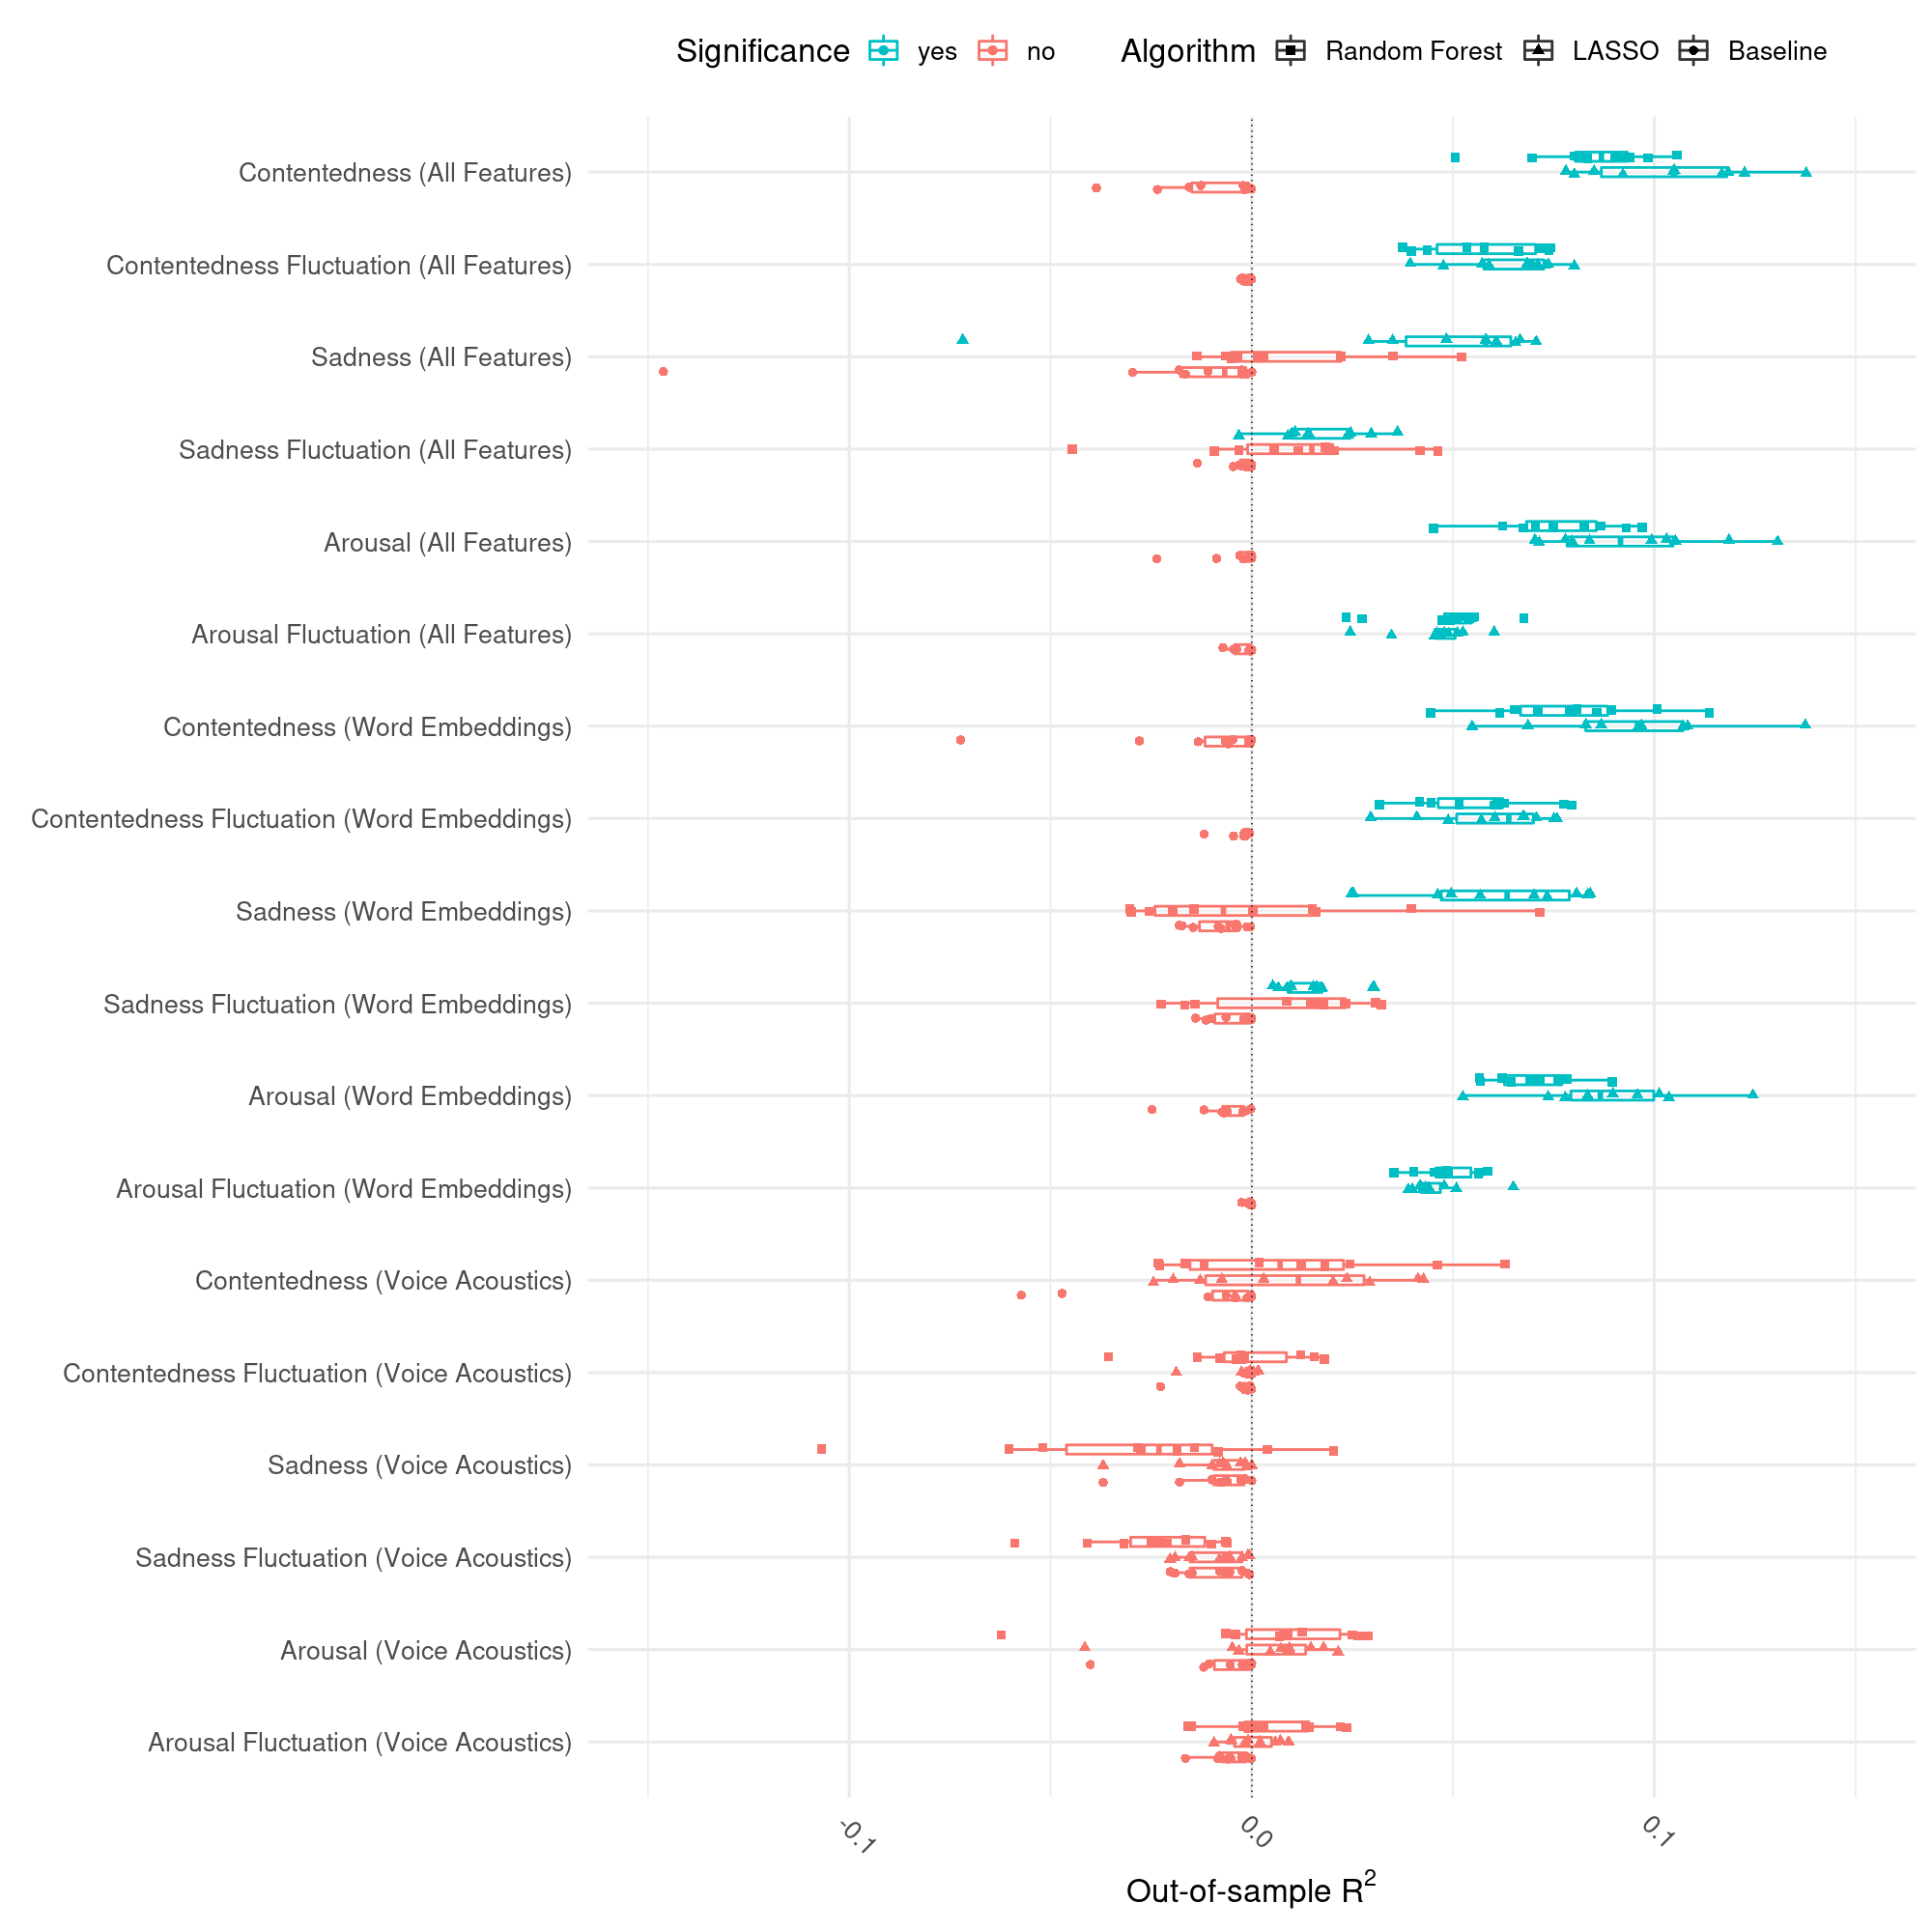
\includegraphics[width=1\linewidth,height=0.9\textheight]{../figures/bmr_us_egemaps_wordembeddings_plot} 

}

\caption[Prediction performance Study 2]{Box and whisker plot of prediction performance measures from 10-fold cross-validation for prediction models in different predictions tasks for each feature (sub) set.}\label{fig:uspredictionoverview}
\end{figure}

\hypertarget{content-effects-on-affect-predictions-from-voice-acoustics-1}{%
\paragraph{Content Effects on Affect Predictions from Voice Acoustics}\label{content-effects-on-affect-predictions-from-voice-acoustics-1}}

In order to exploratively investigate the effect of the emotional valence of the spoken content on affect predictions from voice cues, we used the sentiment score (\emph{M} =0.02, \emph{SD} = 0.29) within the interval of {[}-1; 1{]} that had been assigned to each speech transcript by the Google text-to-speech API. Here, in line with the analysis in Study 1, we analyzed the absolute prediction errors in the prediction of between-person differences in arousal, contentedness, and sadness from voice cues using a Random Forest algorithm. Figure \ref{fig:uscontenteffect} depicts the speech sample's sentiment score on the x-axis and the absolute prediction error on the y-axis.
Result indicate that content sentiment did not have a clear effect on affect predictions from voice cues. Absolute differences in prediction error with varying sentiment were small overall and the predictive performance of the models was generally limited. Possibly, strong negative and positive content sentiment could have reduced the prediction error for arousal and contentedness from voice cues.

\begin{figure}

{\centering 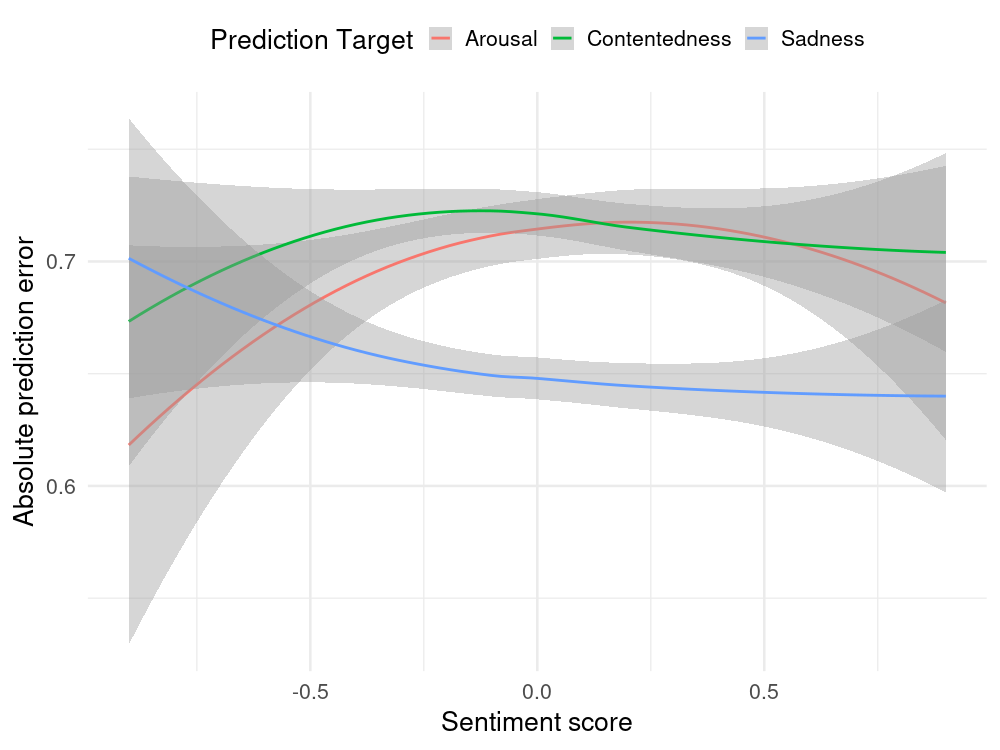
\includegraphics[width=1\linewidth]{../figures/sentiment_error_plot} 

}

\caption[Content sentiment and voice prediction error]{Sentiment score of speech content plotted against the absolute prediction error from Random Forest acoustic predictions}\label{fig:uscontenteffect}
\end{figure}

\newpage

\hypertarget{discussion}{%
\subsection{Discussion}\label{discussion}}

In the present work, we extracted acoustic voice parameters and state-of-the-art word embeddings from speech samples collected using smartphones to predict between-person difference and within-person fluctuations in subjective affect experience. While voice acoustics provided limited predictive information of affective arousal across both studies, speech content had been shown to be predictive of arousal as well valence (sadness and contentedness). Overall, predictions were better when participants could talk freely (versus reading out loud predefined emotional sentences). In our models, we identified loudness and features related to fluctuations of the voice spectrum to be particularly predictive of affective arousal. Finally, experimental (Study 1) and explorative (Study 2) findings suggest that emotional speech content did not affect predictions from voice acoustics (i.e., what someone talks about does not influence how well affect can be predicted from voice cues).

\hypertarget{recognizing-affect-experience-from-speech-cues}{%
\subsubsection{Recognizing Affect Experience from Speech Cues}\label{recognizing-affect-experience-from-speech-cues}}

Our results indicate that speech samples, and particularly their content, allow for the automatic prediction of subjective momentary affect experience. However, our machine learning models achieve a lower prediction performance as reported in prior work on automatic predictions of affect \emph{expression} (Schuller, 2018). Still, our reported performance is similar to studies predicting subjective affect \emph{experience} from speech samples collected in the wild (Carlier et al., 2022; Sun et al., 2020; Weidman et al., 2020). This observation is in line with prior research suggesting that real-life emotions are more difficult to algorithmically recognize than acted or elicited emotions (Vogt et al., 2008). Also, there are only few instances of extreme affect experiences in our data sets compared to the data used in prior studies on acted or labelled emotions. As a result, we rather predicted \emph{mood} in this work, which is, by definition, less intense than emotions (Scherer, 2003) and, consequently, more challenging to recognize.

Furthermore, across the two studies, arousal predictions from voice acoustics were better than those of emotional valence, highlighting prior work showing that the latter is more challenging to automatically infer due to its individual nature (Sridhar \& Busso, 2022). Moreover, in line with prior work (Sun et al., 2020; Weidman et al., 2020), overall predictions of between-person differences in subjective affect experience were superior to those of within-person fluctuations.

Further, as done in prior research on voice-affect predictions (Weidman et al., 2020), we also compared the prediction performance of machine learning models trained on the much larger Compare2016 (6737 features) acoustic feature set (Schuller et al., 2016) in contrast to the economic eGeMAPS (88 features) feature set we had used. Just as in prior research, the larger voice feature set did not yield better affect predictions (Weidman et al., 2020). This finding suggests that an economic acoustic feature set is sufficient for affect detection from voice. Moreover, the small features set is less computationally expensive and would allow for online or on-device pre-processing in a scientific or applied setting.

Generally, our findings challenge the transferability of the optimistic prediction results from prior research work on the recognition of affect \emph{expression} (e.g., enacted speech) to the recognition of subjective affect \emph{experience} in everyday speech, particularly from acoustic voice cues. Thereby, our findings also question the proclaimed performance of commercial affect recognition algorithms deployed in daily life that have been mostly trained on enacted or labelled affect \emph{expression}. Consequently, current expectations regarding the performance of emotion-detecting AI services, especially the ones that are focused on voice cues, applied to everyday speech might be overoptimistic. More research is needed to determine how well algorithms can pick up on subjective affect experience from day-to-day speech.

In future research, smartphone could play a prominent role in collecting and analyzing speech data and corresponding in-situ self-reports on subjective affect experience for affect inferences. Hereby, starting from our work, smartphones could be used as a mobile experimental lab to study different aspects of affect recognition from speech, for example by experimentally varying the content as done in Study 1 (Miller, 2012).

\hypertarget{the-context-of-speech-production-matters}{%
\subsubsection{The Context of Speech Production Matters}\label{the-context-of-speech-production-matters}}

Our results indicate that the context of speech production (i.e., reading out predefined emotional sentences versus prompted free speech) had an impact on affect predictions. While the predefined sentences in Study 1 allowed us to control for the emotionality of the content of participants' voice records, they were unable to express themselves freely, which could have impaired predictions from voice acoustics compared to Study 2 where participants could talk freely. As a result, researchers and practitioners should consider the context in which speech had been produced in and keep in mind that findings and trained models might be specific to the given production context and do not necessarily generalize well to other production contexts.

\hypertarget{the-role-of-speech-content}{%
\subsubsection{The Role of Speech Content}\label{the-role-of-speech-content}}

In Study 2, state-of-the-art word embeddings showed a superior affect prediction performance compared to voice acoustics suggesting that speech content could contain more affective information than speech form. This finding is in line with prior research that found speech content to be more predictive than voice acoustics when predicting momentary subjective experience of happiness (Sun et al., 2020; Weidman et al., 2020). As a consequence, even though prior research has suggested that voice acoustics could be more relevant for human affect inferences than speech content (Ben-David et al., 2016; Lin et al., 2020), future research and AI applications should consider both channels - content and form - simultaneously.

By experimentally varying the emotional valence of the spoken content in Study 1 and exploratively investigating the effect of word sentiment on voice predictions in Study 2, our findings suggest that the content about what participants talked about did not have a substantial impact on affect predictions from voice cues. This insight could imply that it does not matter what people talk about when algorithmically inferring affect experience from voice cues. However, one has to keep than in mind that affect predictions from voice cues were overall not very strong, particularly in Study 1. More research is needed to disentangle speech content and form in automatic affect recognition.

\hypertarget{limitations}{%
\subsection{Limitations and Future Directions}\label{limitations}}

First, we used slightly different operationalizations of affect experience and sample compositions in the two studies that might affect their comparability: In Study 1, we assessed valence and arousal on a six-point Likert scale. In Study 2, we used two items to assess affective valence (contentedness and sadness) and arousal on five-/four-point Likert scales. As a consequence, findings might not be directly comparable. Further, while Study 1 drew on a representative German sample, Study 2 was based on a student convenience sample from the United States with the respective limitations, such as potential constraints in generalizability of findings (Müller, Chen, Peters, Chaintreau, \& Matz, 2021). Also, the German data set that is analyzed in study 1 only contained Android users, excluding those using iOS devices, because of the technical requirements of the logging software. However, past research suggests that the selection bias regarding participant demographics and personality for the German population is negligible (Götz, Stieger, \& Reips, 2017; Keusch, Bähr, Haas, Kreuter, \& Trappmann, 2020; Schoedel et al., 2022). Moreover, both data sets have been collected in Western countries, specifically Germany and the United States. Prior research suggests that there are cultural differences in emotion experience (Lim, 2016) and that mood inference models from sensing data do not necessarily generalize to other countries and cultures (Meegahapola et al., 2023). Future studies should investigate multiple target emotions in diverse international samples from different cultural contexts in non-western countries.

Second, in contrast to prior work using passive speech sensing (e.g., via the EAR), our participants had to actively log their speech in the present work. This artificial setting might have had an effect on results. Moreover, the findings of this study might be subject to the specific instructions that had been given for the audio records: In Study 1, participants were instructed to read out predefined sentences and, in Study 2, participants were prompted to talk about the situation they were in as well as their current thoughts and feelings in a semi-structured fashion. While affect-linked acoustic voice cues in the two studies are similar and are possibly transferable to new voice data, word embeddings are specific to the given task in Study 2. In this manner, future work should employ multiple different speech tasks for affect predictions and investigate how well predictions generalize from one to another.

Also, it should be noted that affective self-reports only from those situations when participants had their smartphone on them and felt comfortable to complete the experience sampling had been analyzed in the present dissertation. Moreover, study participants knew that their affect self-reports and corresponding language samples would be recorded and later analyzed. As a consequence, with regard to assessed subjective affect experience, participants might have only completed the experience sampling questionnaire in selected affective situations, for example not when they were experiencing extreme affective states, or they had not reported on extreme affect at all (Schoedel et al., 2022). Moreover, participants might have not spoken as naturally as they would if they had not known that their data would be scientifically analyzed. Participants might have made the audio records only in selected suitable situations, for example when they were alone in a quiet place. As a result, the resulting data set would also only contain participants' affect experience from being alone in quiet places.

Moreover, specifically to Study 1, another related limitation lies in our privacy-preserving on-device data pre-processing approach. By applying on-device feature extraction, we had no opportunity to check in detail if participants truly complied with study instructions and had recorded their voice while reading out the predefined sentences accordingly (beyond the data-driven quality checks we had applied). Further, our approach did not allow to control for records' background noise (e.g., when participants were outside next to a road) or how they held their smartphone during the voice record. Since checking single raw audio files manually would be out of scope, future research could investigate additional data-driven approaches to check speech data quality directly on the device. Finally, in future work, smartphones could be used to log and immediately pre-process participants' everyday speech by using pre-trained language models to extract content features (e.g., specific topics or word embeddings) directly on the device, too. Thereby, no raw speech data would have to be transferred to a server and valuable information of language's content could be also used for privacy-respectful affect recognition.

Third, the data is comprised of in-situ self-reports of affect experience from participants' everyday life in a non-clinical population. As a result, the data represents the ``normal'' everyday \emph{moods} of regular people with only few cases of extreme positive or negative or very high or low aroused affect experience. As a result, the trained affect recognition models should be considered in this context. If the conducted analyses were to be replicated in a clinical sample that contains more cases of extreme affect experience, findings might be even more distinct. This does not necessarily mean, however, that findings and prediction models from the present dissertation generalize well to a clinical sample. Alternatively, future studies could aim to collect language samples when participants are known to experience strong emotions, for example based on their physiological signals (Hoemann et al., 2020).

Finally, the ground truth, i.e., the information that is assumed to be fundamentally true, used for model training and evaluation are self-reports on participants' subjective affect experience. However, these are prone to response biases (Gao, Saiedur Rahaman, Shao, \& Salim, 2021). These can introduce measurement error that can have a profound impact on the consecutive predictive modeling (Jacobucci \& Grimm, 2020). Moreover, single items were employed to assess state affect experience on different dimensions (i.e., valence and arousal) in the empirical studies. This is an established approach to reduce participant burden by not having them fill out many lengthy experience sampling questionnaires that would also need to be compensated for. However, this single-item approach can introduce additional measurement error for affective responses (Dejonckheere et al., 2022). Future studies that are particularly interested in subjective affect experience should use multiple items assessing a broad range of affect experience in an intensive longitudinal design. Beyond the psychometric challenges associated with using (single item) self-reports to assess momentary affect experience, there is a conceptual debate on how much of an underlying psychological construct, i.e., of affect experience, one can assess using questionnaires. In order to report one's affect experience most accurately through a survey item, one needs to have introspection to recognize it and have an adequate understanding to communicate it accordingly (Boyd, Pasca, \& Lanning, 2020; Montag, Dagum, Hall, \& Elhai, 2022). However, people can vary greatly in that regard (Critchley \& Garfinkel, 2017). Possibly, in the future, algorithms can replace self-report questionnaires altogether by analyzing natural language directly since transformers (that use word embeddings as employed in study 2) have been reported to approach the upper limits in accuracy already (Kjell, Sikström, Kjell, \& Schwartz, 2022).

\hypertarget{conclusion}{%
\subsection{Conclusion}\label{conclusion}}

In this work, we investigated if machine learning algorithms can recognize subjective affect experience from speech samples collected in the wild using smartphones. Extracted acoustic voice parameters provided limited predictive information of affective arousal across both studies, while speech content as reflected in state-of-the-art word embeddings had been shown to be predictive of arousal as well valence (sadness and contentedness). Overall, voice predictions were better when participants could talk freely (versus reading out loud predefined emotional sentences). Also, speech content showed superior prediction performance compared to voice acoustics. Further, experimental and explorative findings suggest that emotional speech content did not affect predictions from voice acoustics (i.e., what someone talked about did not affect how well emotions could be predicted from voice cues). Our findings challenge the transferability of the optimistic prediction results from prior research work and commercial emotion-detection AI algorithms on the recognition of affect \emph{expression} (e.g., enacted and labelled speech) to the recognition of subjective affect \emph{experience} in everyday speech. Finally, we discussed resulting implications for the algorithmic monitoring of affect experience.

\newpage

\hypertarget{references}{%
\section{References}\label{references}}

\hypertarget{refs}{}
\begin{CSLReferences}{1}{0}
\leavevmode\vadjust pre{\hypertarget{ref-banzigerIntroducingGenevaMultimodal2012}{}}%
Bänziger, T., Mortillaro, M., \& Scherer, K. R. (2012). Introducing the {Geneva Multimodal} expression corpus for experimental research on emotion perception. \emph{Emotion (Washington, D.C.)}, \emph{12}(5), 1161--1179. \url{https://doi.org/10.1037/a0025827}

\leavevmode\vadjust pre{\hypertarget{ref-batlinerAutomaticRecognitionEmotions2011}{}}%
Batliner, A., Schuller, B., Seppi, D., Steidl, S., Devillers, L., Vidrascu, L., \ldots{} Amir, N. (2011). The {Automatic Recognition} of {Emotions} in {Speech}. In \emph{Cognitive {Technologies}} (pp. 71--99). \url{https://doi.org/10.1007/978-3-642-15184-2_6}

\leavevmode\vadjust pre{\hypertarget{ref-ben-davidProsodySemanticsAre2016}{}}%
Ben-David, B. M., Multani, N., Shakuf, V., Rudzicz, F., \& van Lieshout, P. H. H. M. (2016). Prosody and {Semantics Are Separate} but {Not Separable Channels} in the {Perception} of {Emotional Speech}: {Test} for {Rating} of {Emotions} in {Speech}. \emph{Journal of Speech, Language, and Hearing Research}, \emph{59}(1), 72--89. \url{https://doi.org/10.1044/2015_JSLHR-H-14-0323}

\leavevmode\vadjust pre{\hypertarget{ref-biecekDALEXExplainersComplex2018}{}}%
Biecek, P. (2018). {DALEX}: {Explainers} for {Complex Predictive Models} in {R}. \emph{Journal of Machine Learning Research}, \emph{19}(84), 1--5.

\leavevmode\vadjust pre{\hypertarget{ref-bischlResamplingMethodsMetaModel2012}{}}%
Bischl, B., Mersmann, O., Trautmann, H., \& Weihs, C. (2012). Resampling {Methods} for {Meta-Model Validation} with {Recommendations} for {Evolutionary Computation}. \emph{Evolutionary Computation}, \emph{20}(2), 249--275. \url{https://doi.org/10.1162/EVCO_a_00069}

\leavevmode\vadjust pre{\hypertarget{ref-boydPersonalityPanoramaConceptualizing2020}{}}%
Boyd, R. L., Pasca, P., \& Lanning, K. (2020). The {Personality Panorama}: {Conceptualizing Personality} through {Big Behavioural Data}. \emph{European Journal of Personality}, \emph{34}(5), 599--612. \url{https://doi.org/10.1002/per.2254}

\leavevmode\vadjust pre{\hypertarget{ref-breimanRandomForests2001}{}}%
Breiman, L. (2001). Random forests. \emph{Machine Learning}, \emph{45}(1), 5--32.

\leavevmode\vadjust pre{\hypertarget{ref-burkhardtDatabaseGermanEmotional2005a}{}}%
Burkhardt, F., Paeschke, A., Rolfes, M., Sendlmeier, W., \& Weiss, B. (2005). \emph{A {Database} of {German Emotional Speech}}. 4.

\leavevmode\vadjust pre{\hypertarget{ref-carlierSearchStateTrait2022}{}}%
Carlier, C., Niemeijer, K., Mestdagh, M., Bauwens, M., Vanbrabant, P., Geurts, L., \ldots{} Kuppens, P. (2022). In {Search} of {State} and {Trait Emotion Markers} in {Mobile-Sensed Language}: {Field Study}. \emph{JMIR Mental Health}, \emph{9}(2), e31724. \url{https://doi.org/10.2196/31724}

\leavevmode\vadjust pre{\hypertarget{ref-critchleyInteroceptionEmotion2017}{}}%
Critchley, H. D., \& Garfinkel, S. N. (2017). Interoception and emotion. \emph{Current Opinion in Psychology}, \emph{17}, 7--14. \url{https://doi.org/10.1016/j.copsyc.2017.04.020}

\leavevmode\vadjust pre{\hypertarget{ref-defrenEmotionalSpeechPerception2018}{}}%
Defren, S., de Brito Castilho Wesseling, P., Allen, S., Shakuf, V., Ben-David, B., \& Lachmann, T. (2018). Emotional {Speech Perception}: {A} set of semantically validated {German} neutral and emotionally affective sentences. \emph{9th {International Conference} on {Speech Prosody} 2018}, 714--718. {ISCA}. \url{https://doi.org/10.21437/SpeechProsody.2018-145}

\leavevmode\vadjust pre{\hypertarget{ref-dejonckheereAssessingReliabilitySingleitem2022}{}}%
Dejonckheere, E., Demeyer, F., Geusens, B., Piot, M., Tuerlinckx, F., Verdonck, S., \& Mestdagh, M. (2022). Assessing the reliability of single-item momentary affective measurements in experience sampling. \emph{Psychological Assessment}, \emph{34}(12), 1138--1154. \url{https://doi.org/10.1037/pas0001178}

\leavevmode\vadjust pre{\hypertarget{ref-eybenGenevaMinimalisticAcoustic2016}{}}%
Eyben, F., Scherer, K. R., Schuller, B. W., Sundberg, J., Andre, E., Busso, C., \ldots{} Truong, K. P. (2016). The {Geneva Minimalistic Acoustic Parameter Set} ({GeMAPS}) for {Voice Research} and {Affective Computing}. \emph{IEEE Transactions on Affective Computing}, \emph{7}(2), 190--202. \url{https://doi.org/10.1109/TAFFC.2015.2457417}

\leavevmode\vadjust pre{\hypertarget{ref-eybenOpensmileMunichVersatile2010}{}}%
Eyben, F., Wöllmer, M., \& Schuller, B. (2010). Opensmile: The munich versatile and fast open-source audio feature extractor. \emph{Proceedings of the International Conference on {Multimedia} - {MM} '10}, 1459. {Firenze, Italy}: {ACM Press}. \url{https://doi.org/10.1145/1873951.1874246}

\leavevmode\vadjust pre{\hypertarget{ref-friedmanRegularizationPathsGeneralized2010}{}}%
Friedman, J., Hastie, T., \& Tibshirani, R. (2010). Regularization paths for generalized linear models via coordinate descent. \emph{Journal of Statistical Software}, \emph{33}(1), 1.

\leavevmode\vadjust pre{\hypertarget{ref-gaoInvestigatingReliabilitySelfreport2021}{}}%
Gao, N., Saiedur Rahaman, M., Shao, W., \& Salim, F. D. (2021). Investigating the {Reliability} of {Self-report Data} in the {Wild}: {The Quest} for {Ground Truth}. \emph{Adjunct {Proceedings} of the 2021 {ACM International Joint Conference} on {Pervasive} and {Ubiquitous Computing} and {Proceedings} of the 2021 {ACM International Symposium} on {Wearable Computers}}, 237--242. {New York, NY, USA}: {Association for Computing Machinery}. \url{https://doi.org/10.1145/3460418.3479338}

\leavevmode\vadjust pre{\hypertarget{ref-gotzUsersMainSmartphone2017}{}}%
Götz, F. M., Stieger, S., \& Reips, U.-D. (2017). Users of the main smartphone operating systems ({iOS}, {Android}) differ only little in personality. \emph{PLOS ONE}, \emph{12}(5), e0176921. \url{https://doi.org/10.1371/journal.pone.0176921}

\leavevmode\vadjust pre{\hypertarget{ref-grimmVeraAmMittag2008}{}}%
Grimm, M., Kroschel, K., \& Narayanan, S. (2008). The {Vera} am {Mittag German} audio-visual emotional speech database. \emph{2008 {IEEE International Conference} on {Multimedia} and {Expo}}, 865--868. \url{https://doi.org/10.1109/ICME.2008.4607572}

\leavevmode\vadjust pre{\hypertarget{ref-hildebrandVoiceAnalyticsBusiness2020}{}}%
Hildebrand, C., Efthymiou, F., Busquet, F., Hampton, W. H., Hoffman, D. L., \& Novak, T. P. (2020). Voice analytics in business research: {Conceptual} foundations, acoustic feature extraction, and applications. \emph{Journal of Business Research}, \emph{121}, 364--374. \url{https://doi.org/10.1016/j.jbusres.2020.09.020}

\leavevmode\vadjust pre{\hypertarget{ref-hoemannContextawareExperienceSampling2020a}{}}%
Hoemann, K., Khan, Z., Feldman, M. J., Nielson, C., Devlin, M., Dy, J., \ldots{} Quigley, K. S. (2020). Context-aware experience sampling reveals the scale of variation in affective experience. \emph{Scientific Reports}, \emph{10}, 12459. \url{https://doi.org/10.1038/s41598-020-69180-y}

\leavevmode\vadjust pre{\hypertarget{ref-huangPredictionEmotionChange2018}{}}%
Huang, Z., \& Epps, J. (2018). Prediction of {Emotion Change From Speech}. \emph{Frontiers in ICT}, \emph{5}.

\leavevmode\vadjust pre{\hypertarget{ref-jacobucciMachineLearningPsychological2020}{}}%
Jacobucci, R., \& Grimm, K. J. (2020). Machine {Learning} and {Psychological Research}: {The Unexplored Effect} of {Measurement}. \emph{Perspectives on Psychological Science}, \emph{15}(3), 809--816. \url{https://doi.org/10.1177/1745691620902467}

\leavevmode\vadjust pre{\hypertarget{ref-keuschCoverageErrorData2020}{}}%
Keusch, F., Bähr, S., Haas, G.-C., Kreuter, F., \& Trappmann, M. (2020). Coverage {Error} in {Data Collection Combining Mobile Surveys With Passive Measurement Using Apps}: {Data From} a {German National Survey}. \emph{Sociological Methods \& Research}, 0049124120914924. \url{https://doi.org/10.1177/0049124120914924}

\leavevmode\vadjust pre{\hypertarget{ref-kjellTextRpackageAnalyzing2021}{}}%
Kjell, O., Giorgi, S., \& Schwartz, H. A. (2021). \emph{Text: {An R-package} for {Analyzing} and {Visualizing Human Language Using Natural Language Processing} and {Deep Learning}}. {PsyArXiv}. \url{https://doi.org/10.31234/osf.io/293kt}

\leavevmode\vadjust pre{\hypertarget{ref-kjellNaturalLanguageAnalyzed2022}{}}%
Kjell, O., Sikström, S., Kjell, K., \& Schwartz, H. A. (2022). Natural language analyzed with {AI-based} transformers predict traditional subjective well-being measures approaching the theoretical upper limits in accuracy. \emph{Scientific Reports}, \emph{12}(1), 3918. \url{https://doi.org/10.1038/s41598-022-07520-w}

\leavevmode\vadjust pre{\hypertarget{ref-knightAmazonWorkingMaking2016}{}}%
Knight, W. (2016). Amazon {Working} on {Making Alexa Recognize Your Emotions}. https://www.technologyreview.com/s/601654/amazon-working-on-making-alexa-recognize-your-emotions/.

\leavevmode\vadjust pre{\hypertarget{ref-kochPredictingAffectiveStates2021}{}}%
Koch, T. K., \& Schoedel, R. (2021). \emph{Predicting {Affective States} from {Acoustic Voice Cues Collected} with {Smartphones}}. \url{https://doi.org/10.23668/psycharchives.4454}

\leavevmode\vadjust pre{\hypertarget{ref-langMlr3ModernObjectoriented2019}{}}%
Lang, M., Binder, M., Richter, J., Schratz, P., Pfisterer, F., Coors, S., \ldots{} Bischl, B. (2019). Mlr3: {A} modern object-oriented machine learning framework in {R}. \emph{Journal of Open Source Software}, \emph{4}(44), 1903. \url{https://doi.org/10.21105/joss.01903}

\leavevmode\vadjust pre{\hypertarget{ref-limCulturalDifferencesEmotion2016}{}}%
Lim, N. (2016). Cultural differences in emotion: Differences in emotional arousal level between the {East} and the {West}. \emph{Integrative Medicine Research}, \emph{5}(2), 105--109. \url{https://doi.org/10.1016/j.imr.2016.03.004}

\leavevmode\vadjust pre{\hypertarget{ref-linProsodyDominatesSemantics2020}{}}%
Lin, Y., Ding, H., \& Zhang, Y. (2020). Prosody {Dominates Over Semantics} in {Emotion Word Processing}: {Evidence From Cross-Channel} and {Cross-Modal Stroop Effects}. \emph{Journal of Speech, Language, and Hearing Research}, \emph{63}(3), 896--912. \url{https://doi.org/10.1044/2020_JSLHR-19-00258}

\leavevmode\vadjust pre{\hypertarget{ref-liuRoBERTaRobustlyOptimized2019}{}}%
Liu, Y., Ott, M., Goyal, N., Du, J., Joshi, M., Chen, D., \ldots{} Stoyanov, V. (2019). \emph{{RoBERTa}: {A Robustly Optimized BERT Pretraining Approach}}. {arXiv}. \url{https://doi.org/10.48550/arXiv.1907.11692}

\leavevmode\vadjust pre{\hypertarget{ref-mandellSpotifyPatentsVoice2020}{}}%
Mandell, J. (2020). Spotify {Patents A Voice Assistant That Can Read Your Emotions}. https://www.forbes.com/sites/joshmandell/2020/03/12/spotify-patents-a-voice-assistant--that-can-read-your-emotions/.

\leavevmode\vadjust pre{\hypertarget{ref-marreroEvaluatingVoiceSamples2022}{}}%
Marrero, Z. N. K., Gosling, S. D., Pennebaker, J. W., \& Harari, G. M. (2022). Evaluating voice samples as a potential source of information about personality. \emph{Acta Psychologica}, \emph{230}, 103740. \url{https://doi.org/10.1016/j.actpsy.2022.103740}

\leavevmode\vadjust pre{\hypertarget{ref-materoEvaluatingContextualEmbeddings2022}{}}%
Matero, M., Hung, A., \& Schwartz, H. A. (2022). Evaluating {Contextual Embeddings} and their {Extraction Layers} for {Depression Assessment}. \emph{Proceedings of the 12th {Workshop} on {Computational Approaches} to {Subjectivity}, {Sentiment} \& {Social Media Analysis}}, 89--94. {Dublin, Ireland}: {Association for Computational Linguistics}. \url{https://doi.org/10.18653/v1/2022.wassa-1.9}

\leavevmode\vadjust pre{\hypertarget{ref-meegahapolaGeneralizationPersonalizationMobile2023}{}}%
Meegahapola, L., Droz, W., Kun, P., de Götzen, A., Nutakki, C., Diwakar, S., \ldots{} Gatica-Perez, D. (2023). Generalization and {Personalization} of {Mobile Sensing-Based Mood Inference Models}: {An Analysis} of {College Students} in {Eight Countries}. \emph{Proceedings of the ACM on Interactive, Mobile, Wearable and Ubiquitous Technologies}, \emph{6}(4), 176:1--176:32. \url{https://doi.org/10.1145/3569483}

\leavevmode\vadjust pre{\hypertarget{ref-mehlElectronicallyActivatedRecorder2017}{}}%
Mehl, M. R. (2017). The {Electronically Activated Recorder} ({EAR}): {A Method} for the {Naturalistic Observation} of {Daily Social Behavior}. \emph{Current Directions in Psychological Science}, \emph{26}(2), 184--190. \url{https://doi.org/10.1177/0963721416680611}

\leavevmode\vadjust pre{\hypertarget{ref-millerSmartphonePsychologyManifesto2012}{}}%
Miller, G. (2012). The {Smartphone Psychology Manifesto}. \emph{Perspectives on Psychological Science: A Journal of the Association for Psychological Science}, \emph{7}(3), 221--237. \url{https://doi.org/10.1177/1745691612441215}

\leavevmode\vadjust pre{\hypertarget{ref-millingSpeechNewBlood2022}{}}%
Milling, M., Pokorny, F., Bartl-Pokorny, K., \& Schuller, B. (2022). Is {Speech} the {New Blood}? {Recent Progress} in {AI-Based Disease Detection From Audio} in a {Nutshell}. \emph{Frontiers in Digital Health}, \emph{4}, 886615. \url{https://doi.org/10.3389/fdgth.2022.886615}

\leavevmode\vadjust pre{\hypertarget{ref-molnarInterpretableMachineLearning2019}{}}%
Molnar, C. (2019). \emph{Interpretable {Machine Learning}}.

\leavevmode\vadjust pre{\hypertarget{ref-montagWeStillNeed2022}{}}%
Montag, C., Dagum, P., Hall, B. J., \& Elhai, J. D. (2022). Do we still need psychological self-report questionnaires in the age of the {Internet} of {Things}? \emph{Discover Psychology}, \emph{2}(1), 1. \url{https://doi.org/10.1007/s44202-021-00012-4}

\leavevmode\vadjust pre{\hypertarget{ref-mullerDepressionPredictionsGPSbased2021}{}}%
Müller, S. R., Chen, X. L., Peters, H., Chaintreau, A., \& Matz, S. C. (2021). Depression predictions from {GPS-based} mobility do not generalize well to large demographically heterogeneous samples. \emph{Scientific Reports}, \emph{11}(1), 14007. \url{https://doi.org/10.1038/s41598-021-93087-x}

\leavevmode\vadjust pre{\hypertarget{ref-nadeauInferenceGeneralizationError2003}{}}%
Nadeau, C., \& Bengio, Y. (2003). Inference for the {Generalization Error}. \emph{Machine Learning}, \emph{52}(3), 239--281. \url{https://doi.org/10.1023/A:1024068626366}

\leavevmode\vadjust pre{\hypertarget{ref-rcoreteamLanguageEnvironmentStatistical2021}{}}%
R Core Team. (2021). \emph{R: {A Language} and {Environment} for {Statistical Computing}}. {Vienna, Austria}: R Foundation for Statistical Computing.

\leavevmode\vadjust pre{\hypertarget{ref-schererVocalCommunicationEmotion2003}{}}%
Scherer, K. R. (2003). Vocal communication of emotion: {A} review of research paradigms. \emph{Speech Communication}, \emph{40}(1-2), 227--256. \url{https://doi.org/10.1016/S0167-6393(02)00084-5}

\leavevmode\vadjust pre{\hypertarget{ref-schoedelSnapshotsDailyLife2022}{}}%
Schoedel, R., Kunz, F., Bergmann, M., Bemmann, F., Bühner, M., \& Sust, L. (2022). \emph{Snapshots of {Daily Life}: {Situations Investigated Through} the {Lens} of {Smartphone Sensing}}. {PsyArXiv}. \url{https://doi.org/10.31234/osf.io/f3htz}

\leavevmode\vadjust pre{\hypertarget{ref-schoedelBasicProtocolSmartphone2020}{}}%
Schoedel, R., \& Oldemeier, M. (2020). \emph{Basic {Protocol}: {Smartphone Sensing Panel Study}}.

\leavevmode\vadjust pre{\hypertarget{ref-schullerSpeechEmotionRecognition2018}{}}%
Schuller, B. (2018). Speech emotion recognition: Two decades in a nutshell, benchmarks, and ongoing trends. \emph{Communications of the ACM}, \emph{61}(5), 90--99. \url{https://doi.org/10.1145/3129340}

\leavevmode\vadjust pre{\hypertarget{ref-schullerINTERSPEECH2016Computational2016}{}}%
Schuller, B., Steidl, S., Batliner, A., Hirschberg, J., Burgoon, J., Baird, A., \ldots{} Evanini, K. (2016). \emph{The {INTERSPEECH} 2016 {Computational Paralinguistics Challenge}: {Deception}, {Sincerity} and {Native Language}} (p. 2005). \url{https://doi.org/10.21437/Interspeech.2016-129}

\leavevmode\vadjust pre{\hypertarget{ref-schwartzEmotionalSpeechProcessing2012}{}}%
Schwartz, R., \& Pell, M. D. (2012). Emotional {Speech Processing} at the {Intersection} of {Prosody} and {Semantics}. \emph{PLoS ONE}, \emph{7}(10), e47279. \url{https://doi.org/10.1371/journal.pone.0047279}

\leavevmode\vadjust pre{\hypertarget{ref-sridharUnsupervisedPersonalizationEmotion2022}{}}%
Sridhar, K., \& Busso, C. (2022). Unsupervised {Personalization} of an {Emotion Recognition System}: {The Unique Properties} of the {Externalization} of {Valence} in {Speech}. \emph{IEEE Transactions on Affective Computing}, \emph{13}(4), 1959--1972. \url{https://doi.org/10.1109/TAFFC.2022.3187336}

\leavevmode\vadjust pre{\hypertarget{ref-sunLanguageWellbeingTracking2020}{}}%
Sun, J., Schwartz, H. A., Son, Y., Kern, M. L., \& Vazire, S. (2020). The language of well-being: {Tracking} fluctuations in emotion experience through everyday speech. \emph{Journal of Personality and Social Psychology}, \emph{118}(2), 364--387. \url{https://doi.org/10.1037/pspp0000244}

\leavevmode\vadjust pre{\hypertarget{ref-vlahosTalkMeHow2019}{}}%
Vlahos, J. (2019). \emph{Talk to {Me}: {How Voice Computing Will Transform} the {Way We Live}, {Work}, and {Think}}. {Eamon Dolan Books}.

\leavevmode\vadjust pre{\hypertarget{ref-vogtAutomaticRecognitionEmotions2008}{}}%
Vogt, T., André, E., \& Wagner, J. (2008). Automatic {Recognition} of {Emotions} from {Speech}: {A Review} of the {Literature} and {Recommendations} for {Practical Realisation}. In C. Peter \& R. Beale (Eds.), \emph{Affect and {Emotion} in {Human-Computer Interaction}} (Vol. 4868, pp. 75--91). {Berlin, Heidelberg}: {Springer Berlin Heidelberg}. \url{https://doi.org/10.1007/978-3-540-85099-1_7}

\leavevmode\vadjust pre{\hypertarget{ref-weidmanNotHearingHappiness2020}{}}%
Weidman, A. C., Sun, J., Vazire, S., Quoidbach, J., Ungar, L. H., \& Dunn, E. W. (2020). ({Not}) hearing happiness: {Predicting} fluctuations in happy mood from acoustic cues using machine learning. \emph{Emotion (Washington, D.C.)}, \emph{20}(4), 642--658. \url{https://doi.org/10.1037/emo0000571}

\leavevmode\vadjust pre{\hypertarget{ref-weningerAcousticsEmotionAudio2013}{}}%
Weninger, F., Eyben, F., Schuller, B. W., Mortillaro, M., \& Scherer, K. R. (2013). On the {Acoustics} of {Emotion} in {Audio}: {What Speech}, {Music}, and {Sound} have in {Common}. \emph{Frontiers in Psychology}, \emph{4}. \url{https://doi.org/10.3389/fpsyg.2013.00292}

\leavevmode\vadjust pre{\hypertarget{ref-wiltingRealVsActed2006}{}}%
Wilting, J., Krahmer, E. J., \& Swerts, M. G. J. (2006). Real vs. Acted emotional speech. \emph{Proceedings of the International Conference on Spoken Language Processing (Interspeech 2006)}.

\leavevmode\vadjust pre{\hypertarget{ref-wrightRangerFastImplementation2017}{}}%
Wright, M. N., \& Ziegler, A. (2017). Ranger: {A Fast Implementation} of {Random Forests} for {High Dimensional Data} in {C}++ and {R}. \emph{Journal of Statistical Software}, \emph{77}(1), 1--17. \url{https://doi.org/10.18637/jss.v077.i01}

\leavevmode\vadjust pre{\hypertarget{ref-wrightLittleInteractionsGet2016}{}}%
Wright, M. N., Ziegler, A., \& König, I. R. (2016). Do little interactions get lost in dark random forests? \emph{BMC Bioinformatics}, \emph{17}(1), 145. \url{https://doi.org/10.1186/s12859-016-0995-8}

\leavevmode\vadjust pre{\hypertarget{ref-wuMultimodalDataCollection2021}{}}%
Wu, C., Fritz, H., Bastami, S., Maestre, J. P., Thomaz, E., Julien, C., \ldots{} Nagy, Z. (2021). Multi-modal data collection for measuring health, behavior, and living environment of large-scale participant cohorts. \emph{GigaScience}, \emph{10}(6). \url{https://doi.org/10.1093/gigascience/giab044}

\leavevmode\vadjust pre{\hypertarget{ref-zouRegularizationVariableSelection2005}{}}%
Zou, H., \& Hastie, T. (2005). Regularization and variable selection via the elastic net. \emph{Journal of the Royal Statistical Society: Series B (Statistical Methodology)}, \emph{67}(2), 301--320. \url{https://doi.org/10.1111/j.1467-9868.2005.00503.x}

\end{CSLReferences}


\end{document}
